\documentclass[a4paper,titlepage]{article}
\usepackage[utf8]{inputenc}
\usepackage[T1]{fontenc} 
\usepackage{geometry}
\usepackage{times}
\geometry{a4paper,left=40mm,right=20mm,top=2cm,bottom=2cm}
\usepackage{graphicx}
\usepackage{amsmath,amsfonts,amssymb}
\usepackage{multirow}
\usepackage{mathtools}
\usepackage{hyperref}
\numberwithin{equation}{section} %Nummeriert mathematische Umgebungen nach sections durch
\usepackage[nodisplayskipstretch]{setspace} %lässt Abstand zwischen align-Umgebungen und Text auf 1.0
\setstretch{1.5}% ergibt 1,5-fachen Zeilenabstand
\usepackage{hyperref}

\begin{document}

\begin{titlepage}
\begin{center}                     
        {\Large\scshape \textbf{Project ML}}\\*[2mm]
				{\large University of Hamburg}\\*[0mm]

				{\large Department of Mathematics}\\*[0mm]
				{\large \emph{Jonas Eckhoff - Timo Greve\\ 
Max Lewerenz - Giulia Satiko Maesaka - John-Robert Wrage}}\\*[30mm]
				

        {\bf \LARGE Machine Learning Methods
         \\ Group 5}\\*[12mm]

\end{center}  

\end{titlepage}
\newpage

%%%%%%%%%%%%%%%%%%%%%%%%%%%%%%%%%%%%%%%%%%%%%%%%%%%%%%%%%
%%%%%%%%%%%%%%%%%%%%%%%%%%%%%%%%%%%%%%%%%%%%%%%%%%%%%%%%%

\pagenumbering{Roman}
\setcounter{page}{2}

\tableofcontents
\newpage

\addcontentsline{toc}{section}{List of figures}
\listoffigures
\newpage

%\addcontentsline{toc}{section}{Tabellenverzeichnis}
%\listoftables
\newpage

%%%%%%%%%%%%%%%%%%%%%%%%%%%%%%%%%%%%%%%%%%%%%%%%%%%%%%%%%
%%%%%%%%%%%%%%%%%%%%%%%%%%%%%%%%%%%%%%%%%%%%%%%%%%%%%%%%%

\pagenumbering{arabic}
\setcounter{page}{1}

\section{Introduction}

These notes are the documentation of the research on machine learning methods lead during the development of an engine for facial emotion recognition for the course on Machine Learning at the University of Hamburg. This document aims to give an overview on the current context of Machine Learning and then it focuses on presenting the algorithms implemented in the engine (KNN, SVM, AdaBoost and CNN); it explains how they work, their advantages and disadvantages.
\section{What is ML?}

Machine learning is the field of study responsible for developing and understanding algorithms that allow computer systems to perform certain tasks independently. The type of tasks considered are these for which any rule-based approach is unfeasible, either because a precise set of rules is unclear, for example in pattern recognition, or because computing according to the rules is too complex, for example in playing Go. 

Given a data set, the goal of a machine learning method can be of two types, one is to use the data to find a function, which will then match new input data to a value; another is to find a subdivision of the data set based on similarities. The methods used for the first type of goal are named \textit{supervised learning} methods and the given data set, called \textit{training set}, must be structured in pairs input-output. For the second type of goal, one uses \textit{unsupervised learning} methods.  

In a supervised learning method, the output value is either quantitative or qualitative. For the problem of predicting the price of house given its area and location, the output is a quantitative value; these are called \textit{regression} problems. On the other hand, if the task is to address an emotion to a given face expression, the output is a qualitative value encoding a certain emotion; these are called \textit{classification} problems.

Supervised learning methods are structured in two parts. Firstly it consists of a predetermined set of functions, called \textit{hypothesis space}, from which a final function will be chosen. Secondly the method needs a predetermined way of searching through the hypothesis space, therefore it requires a predetermined \textit{loss function} and \textit{optimization algorithm}. The choice of hypothesis space, loss function and optimization algorithm depends on the task and different methods need to be implemented and evaluated. For the task of recognizing facial emotion, it is known that between the methods so far developed, the best results are achieved by convolutional neural networks. Still, this project tests different methods one more time, for the sake of experience.

\begin{figure}[hbtp]
	\centering
	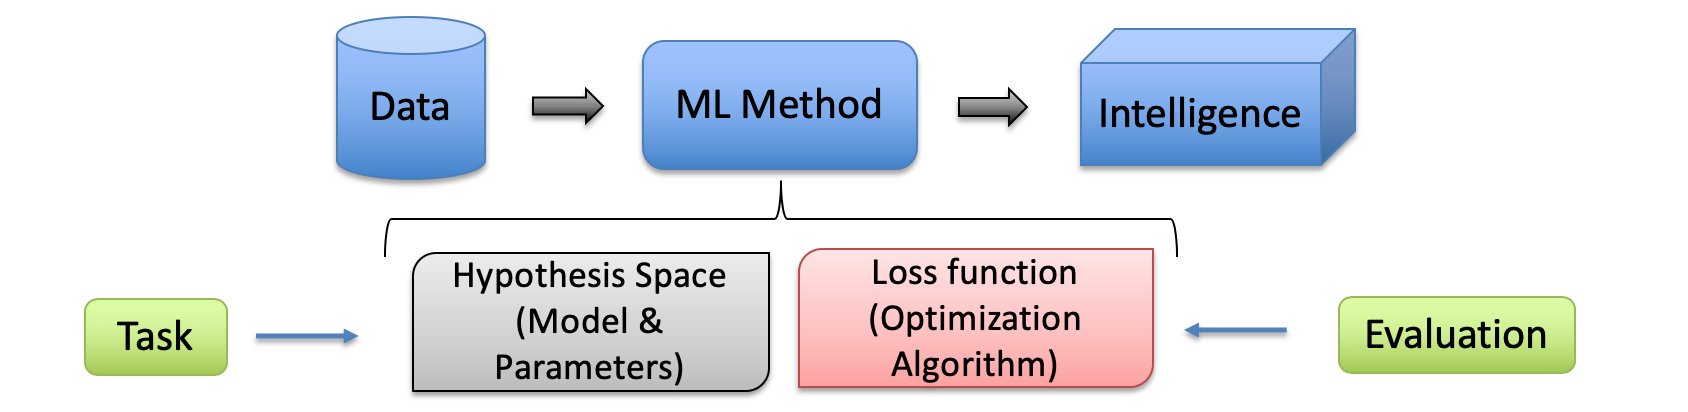
\includegraphics[width=1\textwidth]{./Images/MLPipe}
	\caption{The flow of developing an engine based on machine learning.}
	% \vspace{-20pt}
	\label{fig:Datensatz - unbearbeitet}
\end{figure}

\begin{figure}[hbtp]
	\centering
	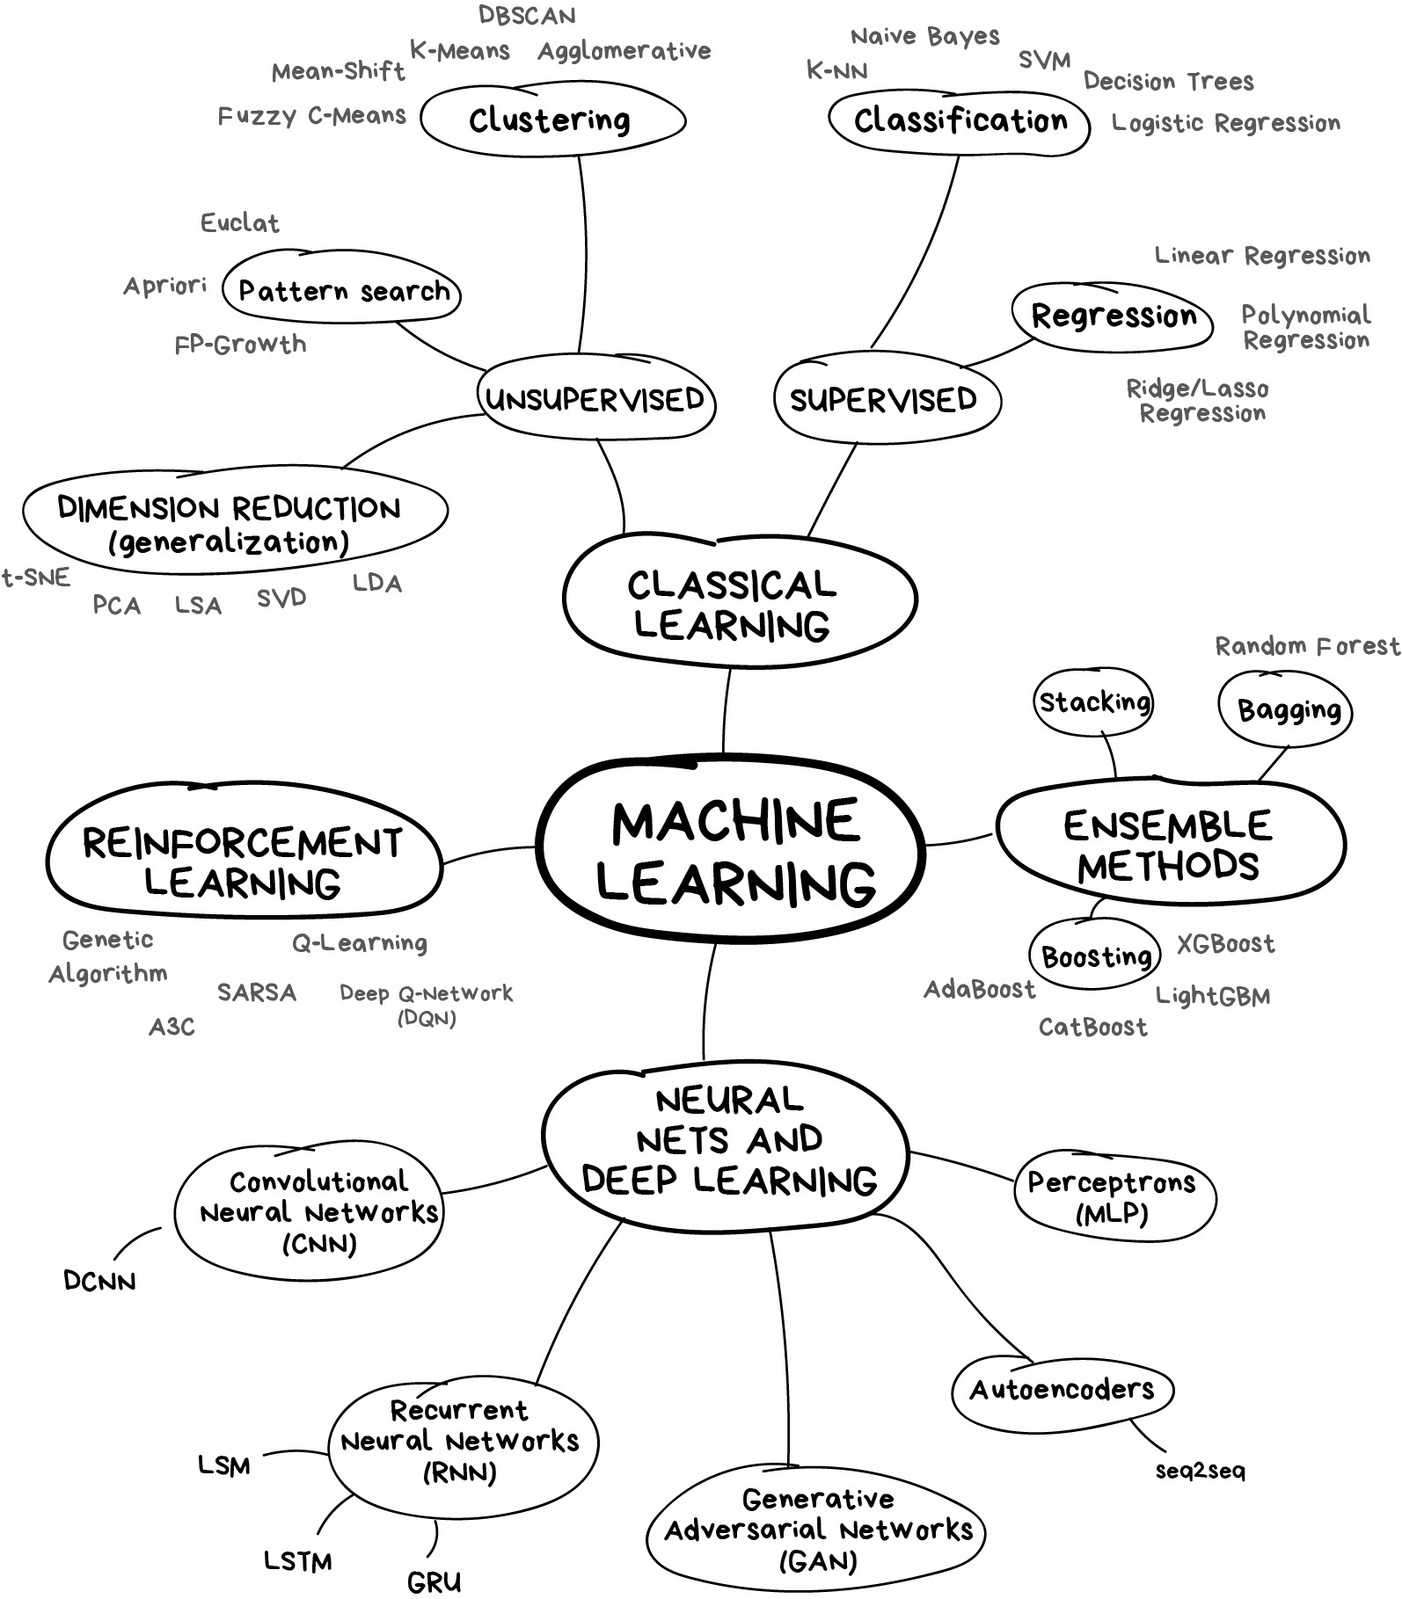
\includegraphics[width=1\textwidth]{ML}
	\caption{ML-Overview}
	% \vspace{-20pt}
	\label{fig:Datensatz - unbearbeitet}
\end{figure}


\newpage
\section{Classical learning}
In this Chapter 3 we are going to explain the methods k-nearest-neighbours and support vector machine. Also we are going to briefly introduce decision trees because we are using them in Chapter 5 for AdaBoost.

%%%%%%%%%%%%%%%%%%%%%%%%%%%%%%%%%%%%%%%%%%%%%%%%%%%%%%%%%

\subsection{KNN}
The KNN algorithm assumes that similar things exist in close proximity. In other words, similar things are near to each other.

The straight-line distance (Euclidean distance) is a popular and familiar choice to measure the distance between two samples.
Note that there are other ways of calculating distance, and one way might be preferable depending on the problem we are solving. Other possibilities to measure the distance could be e.g. Manhattan or Hamming.
In the following picture the black dot could be classified as - if we only compare with the next neighbour. But if one chooses to compare with the three nearest neighbours, the dot would be classified as +, because two dots would be + and only one would be -. It is important to select a "good" amount of neighbours to classify. An example for this can be found in the next picture where the black dot is near to a (probably) outlier. If k would be chosen as 1 then the black dot would be classified as + but it would probably be -.

\begin{figure}[hbtp]
	\centering
	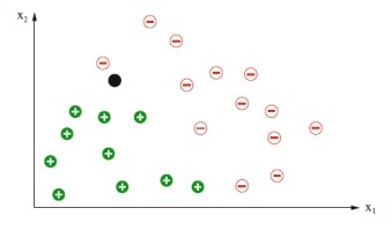
\includegraphics[scale=0.8]{knn1}
	\caption{K-Nearest Neighbors}
	% \vspace{-20pt}
	\label{fig:Datensatz - unbearbeitet}
\end{figure}

\begin{figure}[hbtp]
	\centering
	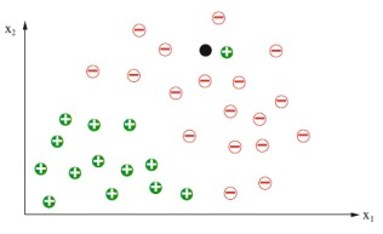
\includegraphics[scale=0.8]{knn2}
	\caption{K-Nearest Neighbors}
	% \vspace{-20pt}
	\label{fig:Datensatz - unbearbeitet}
\end{figure}
 
 
\textbf{Sources:}
\begin{itemize}
\item scikit-learn: \hyperlink{https://scikit-learn.org/stable/modules/generated/sklearn.neighbors.KNeighborsClassifier.html}{https://scikit-learn.org/stable/modules/generated/sklearn.neighbors.KNeighborsClassifier.html} \\
\hyperlink{https://scikit-learn.org/stable/modules/neighbors.html}{https://scikit-learn.org/stable/modules/neighbors.html}
\item Wikipedia: Nächste-Nachbarn-Klassifikation \hyperlink{https://de.wikipedia.org/wiki/Nächste-Nachbarn-Klassifikation}{https://de.wikipedia.org/wiki/Nächste-Nachbarn-Klassifikation}
\end{itemize} 
%%%%%%%%%%%%%%%%%%%%%%%%%%%%%%%%%%%%%%%%%%%%%%%%%%%%%%%%%

\subsection{Decision Trees}

(Classification-) Decision tree

The data will be divided by yes/no questions. This is done by selecting the question such that the best information gain is created (splitting the data via a feature which can separate the different labels best). There are different methods to measure the entropy from which the information gain can be calculated. A common approach is to calculate the Gini-index. For more information please have a look at the sources. In the following picture one can see a decision tree with depth 8. Trees tend to overfit if one let them grow to their maximum depth, so there are methods to prevent this from happening (e.g. pruning).

\begin{figure}[hbtp]
	\centering
	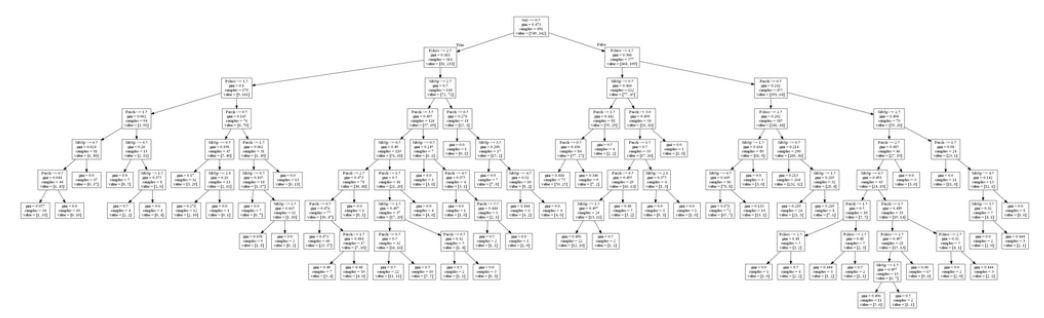
\includegraphics[scale=0.5]{tree}
	\caption{Decision Tree}
	% \vspace{-20pt}
	\label{fig:Datensatz - unbearbeitet}
\end{figure}


Decision Trees can be used for ensemble methods (Random forest, AdaBoost,...). We refer to Chapter 5.

\textbf{Sources:}
\begin{itemize}
\item scikit-learn: \hyperlink{https://scikit-learn.org/stable/modules/tree.html}{https://scikit-learn.org/stable/modules/tree.html} \\
\hyperlink{https://scikit-learn.org/stable/modules/generated/sklearn.tree.DecisionTreeClassifier.html}{https://scikit-learn.org/stable/modules/generated/sklearn.tree.DecisionTreeClassifier.html}
\item Wikipedia: Entscheidungsbaum \hyperlink{https://de.wikipedia.org/wiki/Entscheidungsbaum}{https://de.wikipedia.org/wiki/Entscheidungsbaum}
\end{itemize}

%%%%%%%%%%%%%%%%%%%%%%%%%%%%%%%%%%%%%%%%%%%%%%%%%%%%%%%%%%%
%%%%%%%%%%%%%%%%%%%%%%%%%%%%%%%%%%%%%%%%%%%%%%%%%%%%%%%%%%%
\subsection{Support Vector Machine}
\subsubsection{Introduction}

Support Vector Machines (SVM) are supervised learning algorithms for classification.
They are one of the most widely used supervised learning algorithms. 
SVMs offer a high accuracy when it comes to classification.
The idea behind a SVM is to find a hyperplane that seperates classes of datapoints with a large margin. Where the margin is the smallest distance between the closest datapoint $x$ of one class and the hyperplane (therefore the name 'support vector'). Because of this feature the SVM is sometimes also called \textbf{large margin classifier}.
The so called kernel trick can be applied when non linear data has to be classified.

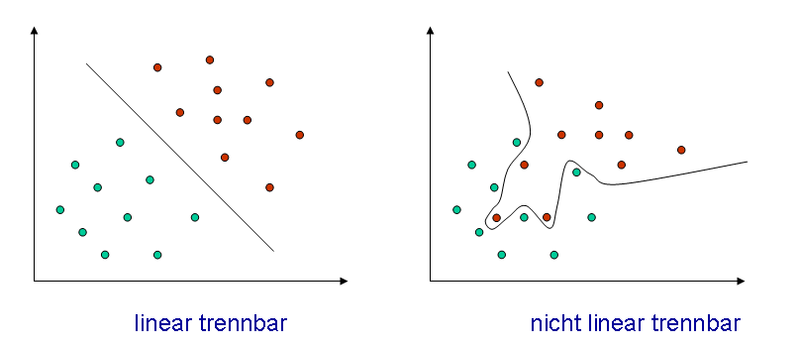
\includegraphics[scale=0.5]{Images/svm.png}


\subsubsection{Linear Support Vector Machines}

For a smooth start, assume the Support Vector Machine algorithm is being used for a binary classification problem~$\mathcal{Y} = \{-1, 1\}$, that the training set has~$\mathcal{X} \subset \mathbb{R}^d$ and the subsets~$X_{-1} = \{ x^i\in \mathcal{X} \colon y^i = -1 \}$, ~$X_{1} = \{ x^i\in \mathcal{X} \colon y^i = 1 \}$ can be the separated by an affine hyperplane. Under these assumptions, the hypothesis space is the set of affine hyperplanes in~$\mathbb{R}^d$ that separate the training data and not all possible affine hyperplanes, as in Linear regression.

While in Linear Regression the empirical risk adds an error for each element in the data set, in SVMs the error of a given hyperplane is the sum~$\delta_{-} + \delta_{+}$, where~$\delta_{-}$ is the minimum distance between the hyperplane and an input point which would be classified as~$-1$ and~$\delta_{+}$ is defined analogously, for an input point which would be classified as~$1$.


\subsubsection{Mathematics behind SVMs}
For given input data $X = \{x_{1}, ..., x_{m}\}$, with $x_{i} \in \mathbb{R}^n$ and matching result vector $Y = \{y_{1}, ..., y_{m}\}$, with $y_{i} \in \{-1, 1\}$. We want a classifier \\ $h: \mathbb{R}^{n} \rightarrow \{-1, 1\}$ such that $h(x) = $ $\begin{cases*} 1 & ,if $ w^{T} x + b  > 0$,\\ -1& ,if $w^{T} x+b < 0$.\end{cases*}$ with $w \in \mathbb{R}^{n}$ and $b \in \mathbb{R}$. We want $h$ to be correct for most samples. This formulation leads to the following primal problem: \\
$min_{w,b,s} \frac{1}{2} w w^T + C \sum_{i = 1}^m s_{i}$, \\
s.t.: $y_i (w^T x_i + b ) \geq 1 - s_i$, $s_i \geq 0$. \\
Where $s_i$ are the so called slack variables that should denote the distance from the correct margin if a point is misclassified. \\
Intuitively we want to maximize the margin what results in minimizing $||w||^2$ including a penalty when something is misclassified.
$C$ controls the strength of the misclassification penalty. One could view it as a inverse regularization parameter. A large $C$ results in overfitting and a smaller $C$ results in a "smoother" fit.\\
The dual problem to the above Primal problem is: \\
$min_{\lambda} \frac{1}{2} \lambda^T Q \lambda - e^T \lambda$ \\
s.t.: $y^T \lambda = 0$ and $0 \leq \lambda_{i} \leq C$ for all $i = 1,...,m$.
The entries of the matrix $Q \in \mathbb{R}^{m \times m}$ are given by $Q_{i, j} = y_i y_j \langle x_i, x_j \rangle$. \\
This shows that the minimization only depends on the scalar product of $x_i$ and $x_j$ and we can apply the kernel trick. Instead of the standard scalar product, we can use a kernel function $K(x_i, x_j)$.

\subsubsection{In our case}
We use the python library sklearn, which can easily be installed via pip.
First we get the training data and split it into training and test data.\\
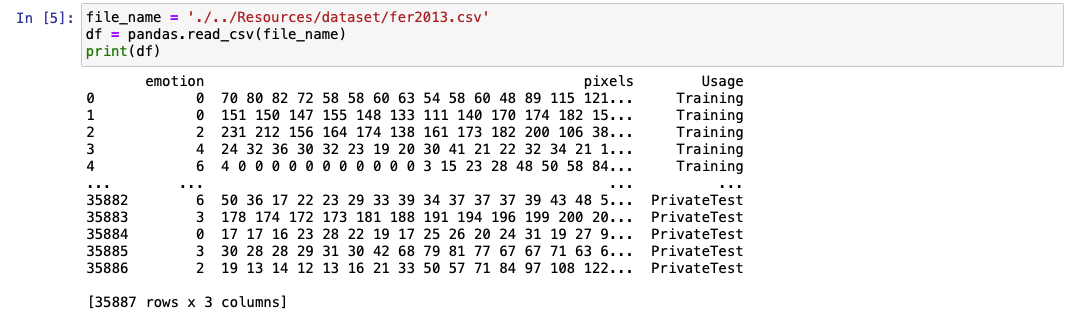
\includegraphics[scale=0.4]{Images/trainingdata.png} \\
Next we fit the model to the training data for the chosen parameters and safe it with the pickle model. \\
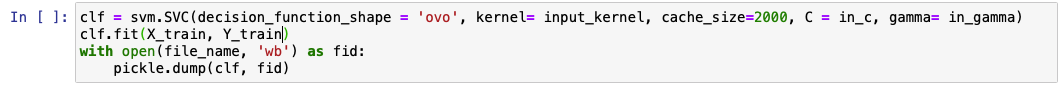
\includegraphics[scale=0.4]{Images/trainmodel.png} \\
Now the model can give a prediction on new images. \\
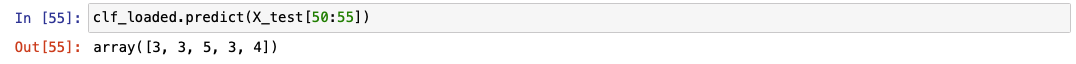
\includegraphics[scale=0.4]{Images/svm_prediction.png}

\textbf{Sources:}
\begin{itemize}
\item Martin Lotz: \textit{Mathematics of Machine Learning}. Lecture Notes, Warwick (UK), 2020.
\item scikit-learn: \hyperlink{https://scikit-learn.org/stable/modules/generated/sklearn.svm.SVC.html}{https://scikit-learn.org/stable/modules/generated/sklearn.svm.SVC.html} \\
\hyperlink{https://scikit-learn.org/stable/modules/svm.html}{https://scikit-learn.org/stable/modules/svm.html}
\item Coursera: Machine Learning, by Stanford University \\ \hyperlink{https://www.coursera.org/learn/machine-learning/home/welcome}{https://www.coursera.org/learn/machine-learning/home/welcome}
\item Wikipedia: Support vector machine.\hyperlink{https://en.wikipedia.org/wiki/Support\_vector\_machine}{https://en.wikipedia.org/wiki/Support\_vector\_machine}
\end{itemize}


%%%%%%%%%%%%%%%%%%%%%%%%%%%%%%%%%%%%%%%%%%%%%%%%%%%%%%


\newpage
\section{Neural Networks and Deep Learning}


\subsection{Convolutional Neural Networks CNN}

A Convolutional Neural Network is a Deep Learning algorithm which is primarily used to classify images. It can more easily capture spatial (and temporal) dependencies since the convolution filters use a linear combination of neighboring pixels to calculate an output value. After a convolution filter is applied, a Max-Pooling filter can be applied, which lowers the amount of nodes in the network. A $2$x$2$ Max-Pooling filter, for example, replaces every $2$x$2$ square with the maximal value in that square, resulting in lowering the amount of nodes after that layer to a quarter.
At the end the multidimensional layers are flattened to a one dimensional vector that is connected to the output via a fully connected layer.

\begin{figure}[hbtp]
	\centering
	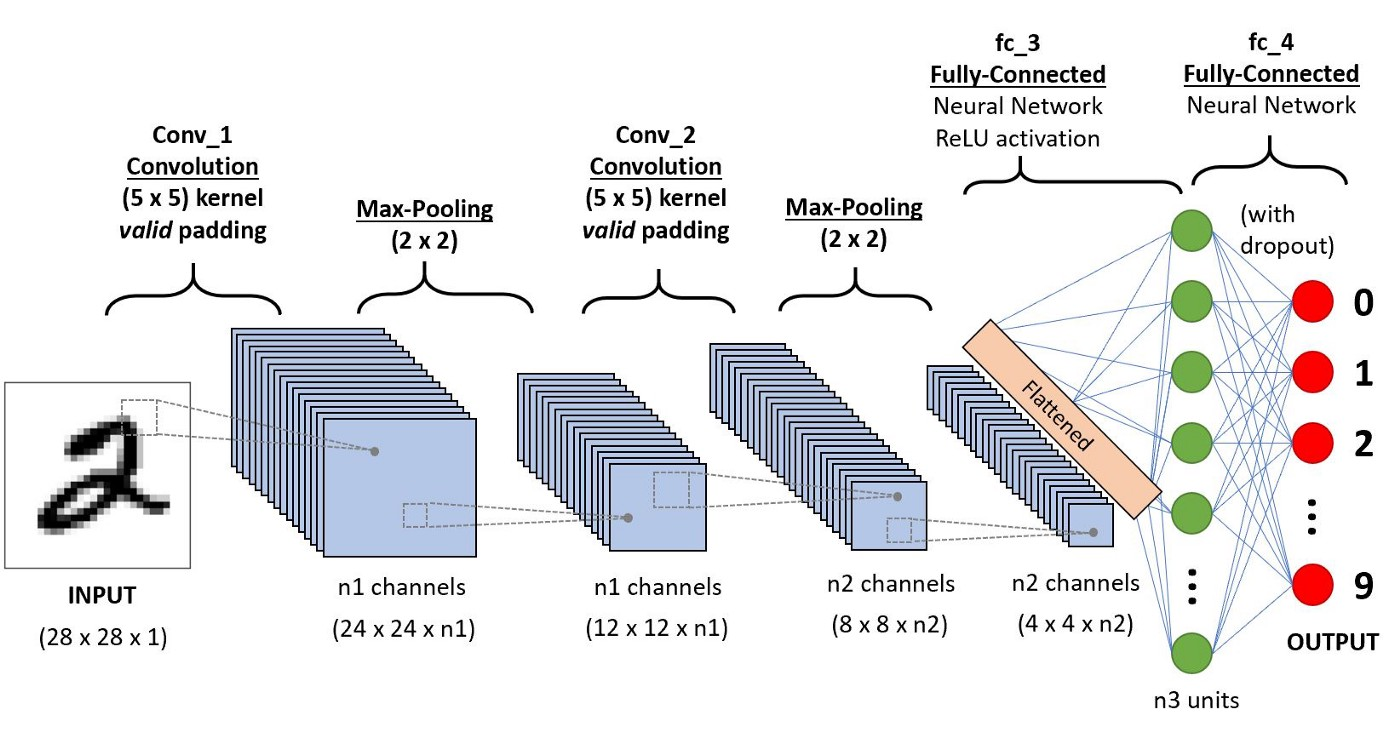
\includegraphics[width=1\textwidth]{Images/CNN}
	\caption{Example of a CNN architecture}
\end{figure}

Helpful links:\\
A Comprehensive Guide to Convolutional Neural Networks — the ELI5 way
\\
\url{https://towardsdatascience.com/a-comprehensive-guide-to-convolutional-neural-networks-the-eli5-way-3bd2b1164a53}
\\

Since we want to detect emotions in images, a convolutional neural network would be a good choice. It is the go-to type of network for these kind of computer vision problems.

\subsection{Recurrent Neural Networks RNN}

A recurrent neural network (RNN) is a type of artificial neural network commonly used in speech recognition and natural language processing. It uses feedback loops, that allow information to persist (the network has memory), to process sequences of data.\\

RNNs are not useful to analyse facial expression in an image.

\subsection{Generative adversarial networks GAN}

Generative adversarial networks (GANs) are algorithmic architectures that use two neural networks, pitting one against the other in order to generate new, synthetic instances of data that can pass for real data. They are used widely in image generation, video generation and voice generation.\\
One neural network, called the generator, generates new data instances, while the other, the discriminator, evaluates them for authenticity; i.e. the discriminator decides whether each instance of data that it reviews belongs to the actual training dataset or not.\\

Helpful links:\\
A Beginner's Guide to Generative Adversarial Networks (GANs)
\\
\url{https://pathmind.com/wiki/generative-adversarial-network-gan}
\\

GANs can be used to generate images and videos. We could use this type of network to expand training data. 
Having a well trained GAN would allow us to create new images for specific emotions that look convincingly real in order to prevent overfitting by creating an endless stream of new images. 
It may also be used to create video training data that can be used to train a neural network with memory to better capture changes in emotion in a video stream. 
The training of a GAN however takes a very long time compared to a simple CNN which makes it probably unfeasible for us even though it would create interesting possibilities to explore. 


\subsection{Autoencoders}

Autoencoders are a specific type of feedforward neural networks where the input is the same as the output. They compress the input into a lower-dimensional code and then reconstruct the output from this representation. The code is a compact “summary” or “compression” of the input.
An autoencoder consists of 3 components: encoder, code and decoder. The encoder compresses the input and produces the code, the decoder then reconstructs the input only using this code.

\begin{figure}[hbtp]
	\centering
	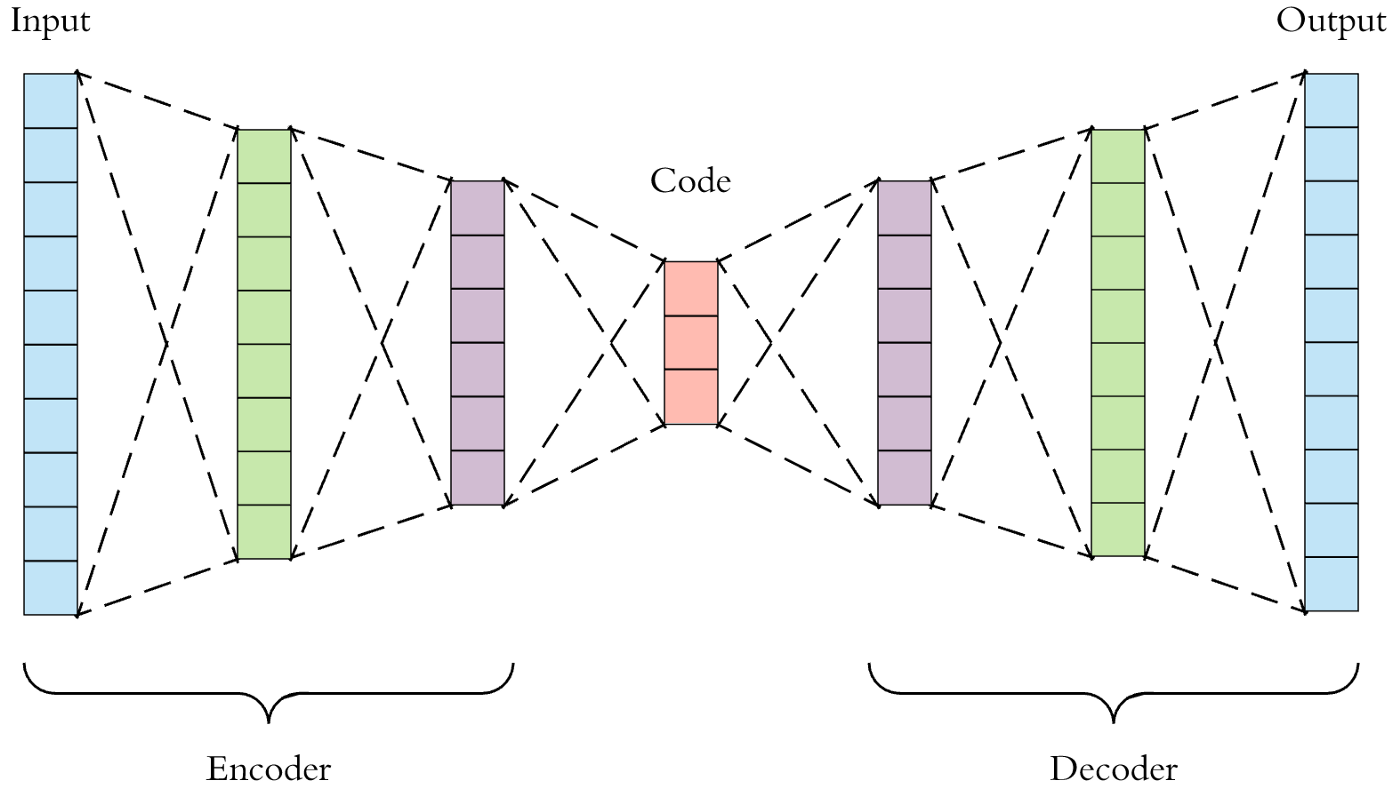
\includegraphics[width=1\textwidth]{Images/Autoencoder}
	\caption{Example of an autoencoder architecture}
\end{figure}

Helpful links:\\
Applied Deep Learning - Part 3: Autoencoders
\\
\url{https://towardsdatascience.com/applied-deep-learning-part-3-autoencoders-1c083af4d798}\\

An autoencoder is used to reduce the dimensionality. Since there is a lot of redundancy in images, especially if they all contain more or less centered faces, it can be expected that an autoencoder could shrink the input size considerably before using a different neural network. This could potentially make the training process a lot quicker. We would however not be able to use a convolutional neural network anymore because the 2 dimensional image structure is lost by removing the redundancy with the autoencoder. Moreover some information may be lost in the process which could affect the overall accuracy of the neural network. 

The effectiveness of an autoencoder could possibly be explored if there are given time constraints for the training process. It can also be compared to principal component analysis (PCA) which removes redundancy in a more controlled way. 

%\subsection{Perceptrons MLP}


%%%%%%%%%%%%%%%%%%%%%%%%%%%%%%%%%%%%%%%%%%%%%%%%%%%%%%%%%


\newpage
\section{Ensemble Methods}
The main idea of ensemble is to combine algorithms to achieve a better accuracy than with a single model. Ensemble methods can be split into heterogeneous and homogeneous ensembles. In homogeneous ensembles only one classifier is used, while in heterogeneous ensembles different algorithms can be combined. 
We implemented a homogeneous method called AdaBoost with decision tree stumps (depth=1). This is a boosting method. There are other fields like Bagging (Bootstraping) or Random Forest which are not explained here. For a first introduction with Desicion Trees you can look at https://medium.com/analytics-vidhya/ensemble-methods-for-decision-trees-f4a658af754d.\\
\begin{figure}[hbtp]
	\centering
	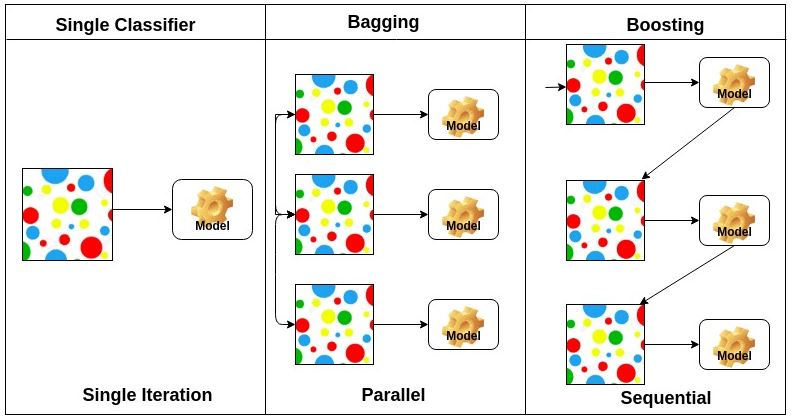
\includegraphics[scale=0.5]{ensemble_1}
	\caption{Bagging/Boosting}
	% \vspace{-20pt}
	\label{fig:Datensatz - unbearbeitet}
\end{figure}
If we consider decision trees, we can observe that they tend to overfit if they grow to their maximum depth. Also in every node there is uncertainty. Ensemble methods try to build a bunch of weak learner (like the mentioned stumps) to let them predict together and try to decrease variance (and bias).

%%%%%%%%%%%%%%%%%%%%%%%%%%%%%%%%%%%%%%%%%%%%%%%%%%%%%%%%%


\subsection{AdaBoost}
For our problem we implemented an algorithm called AdaBoost. The main idea behind AdaBoost is building a series of trees, each of those being an updated version of the previous one. At the end of the process, when all the classifiers built during the iterations will be asked to vote for the target of a new observation, there will be trees with a heavier vote than others. Those are the trees that performed the best during all the iterations (so, they showed very few misclassifications).

- AdaBoost works by putting more weight on difficult to classify instances and less on those already handled well.

Like mentioned we implemented AdaBoost with Stumps (depth=1). Regarding the functionality of Decision Trees we refer to Chapter 3 Classical learning. The input was the same like for the other algorithms (2304 pixels) and the emotions. The process of the algorithm can be seen in the following graphic. 
\begin{figure}[hbtp]
	\centering
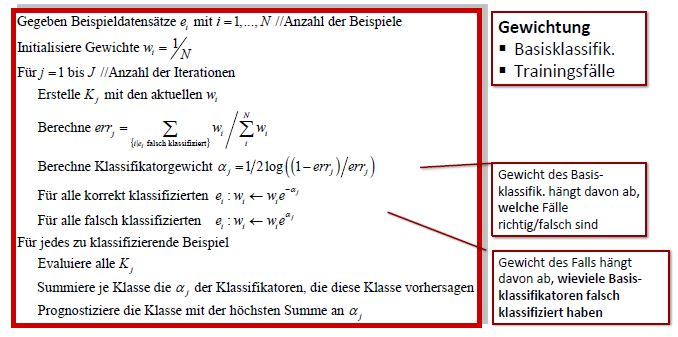
\includegraphics[scale=0.8]{Images/Adaboost_1.png} \\
\end{figure}

In summary it can be said that AdaBoost had a surprisingly good accuracy compared with SVM. But the algorithm tends to classify a lot of pictures as happy and is weak at classifying Angry, Disgust and Fear.\\
One advantage of AdaBoost is that it is easily implemented and the training is rather simple. It is also possible to use different weak learner (Trees, KNN, etc.) But if the weak learner selected doesn't fit the problem, then AdaBoost also struggles solving it. Also with growing iterations AdaBoost can overfit. Another disadvantage is that, due to the iterative calculation, it's difficult to parallelize.

\textbf{Sources:}
\begin{itemize}
\item Introduction to AdaBoost \hyperlink{https://towardsdatascience.com/understanding-adaboost-for-decision-tree-ff8f07d2851}{https://towardsdatascience.com/understanding-adaboost-for-decision-tree-ff8f07d2851}
\item scikit-learn: \hyperlink{https://scikit-learn.org/stable/modules/ensemble.html}{https://scikit-learn.org/stable/modules/ensemble.html} \\
\hyperlink{https://scikit-learn.org/stable/modules/generated/sklearn.ensemble.AdaBoostClassifier.html}{https://scikit-learn.org/stable/modules/generated/sklearn.ensemble.AdaBoostClassifier.html}
\item Video with an example \\ \hyperlink{https://www.youtube.com/watch?v=LsK-xG1cLYA}{https://www.youtube.com/watch?v=LsK-xG1cLYA}
\item Wikipedia: Boosting \hyperlink{https://de.wikipedia.org/wiki/Boosting}{https://de.wikipedia.org/wiki/Boosting}
\end{itemize}

%%%%%%%%%%%%%%%%%%%%%%%%%%%%%%%%%%%%%%%%%%%%%%%%%%%%%%%%%


\newpage
\section{Reinforcement learning}


\newpage

\begingroup
\addcontentsline{toc}{section}{Bibliography}
\renewcommand*\refname{Bibliography}

\begin{thebibliography}{----}
% Check - Korrekt 

\bibitem{Deutsche Aktuarvereinigung e.V.}
\textsc{Deutsche Aktuarvereinigung e.V.}, 2012: Unisex-Tarifierung, abgerufen am 10. November 2019: https://aktuar.de/fachartikelaktuaraktuell/Lebensversicherung{\_}Unisex{\_}Aktuar-aktuell{\_}19.pdf{\#}search=unisex

\bibitem{Ertel2016}
\textsc{Ertel}, W. (2016): {\it Grundkurs Künstliche Intelligenz}. Springer Vieweg, Wiesbaden. 4. Auflage.


\end{thebibliography}
\endgroup


\newpage


\end{document}
